\documentclass[11pt,a4paper,titlepage,openany,oneside]{book}
\usepackage[utf8]{inputenc}
\usepackage[T1]{fontenc}
\usepackage[french]{babel}
\usepackage[top=1.5cm, bottom=4cm]{geometry}
\usepackage{fancyhdr, graphicx, array, hyperref}

\pagestyle{fancy}

\title{\textsc{\textbf{Manuel utilisateur\\Interpréteur du langage LIR}}}
\date{}
\author{Nicolas \textsc{Caminade} \and
        Sylvan \textsc{Courtiol} \and
        Pierre \textsc{Debas} \and
        Heïa \textsc{Dexter} \and
        Lucàs \textsc{Vabre} }

\begin{document}

    \renewcommand\sfdefault{pag}

    \lhead{\leftmark}
    \rhead{
        
\includegraphics[width=2cm]{img/logoiut}
    }

    \cfoot{\thepage}
    \headheight = 2cm
    \headsep = 0.5cm

    \begin{titlepage}
        \fontfamily{pag}\selectfont

        \begin{center}\normalsize
            \MakeUppercase{IUT de Rodez \hfill Département informatique
                \hfill INFO1 2020-2021}
        \end{center}
        \vspace*{0.1cm}
        \hrule
        \vspace*{0.2cm}
        \begin{flushright}
            
\includegraphics[width=4cm]{img/logoiut}
        \end{flushright}
        \vspace*{2cm}
        \begin{flushright}\Huge
            \textsc{\textbf{Manuel utilisateur\\Interpréteur du langage LIR}}
        \end{flushright}
        \hrule
        \begin{flushleft}
            \MakeUppercase{Projet proposé par Frédéric Barrios}
        \end{flushleft}
        \vspace*{2cm}
        \begin{center}\Large
            Nicolas \textsc{Caminade}, Sylvan \textsc{Courtiol},\\
            Pierre \textsc{Debas}, Heïa \textsc{Dexter}, \\
            Lucàs \textsc{Vabre}
        \end{center}
        \vfill
        \begin{center}\normalsize
            \MakeUppercase{Projet tuteuré --- Semestre 2}
        \end{center}
    \end{titlepage}

    \renewcommand\rmdefault{pag}
    \fontfamily{pag}\selectfont
    \renewcommand{\sfdefault}{pag}
    %\renewcommand{\ttdefault}{pag}


    % Sommaire
    \renewcommand{\contentsname}{Sommaire}
    \tableofcontents

    % TODO Plan

    \chapter{Installation}
        \section{Pré-requis}
    \paragraph{JDK (Java Development Kit)}
    Pour un système d'exploitation Windows, l'utilisation de
    l'interpréteur LIR nécessite le jdk-15 ou une version ultérieure.

    \subsection{Installer le jdk-15}
    Sur la plateforme en ligne \verb|https://openjdk.java.net/projects/jdk/|,
    dans la rubrique "Release", télécharger la dernière version disponible du
    jdk.
    \\ Ranger le fichier .ZIP dans votre arborescence. Extraire les fichiers.

    \begin{center}
        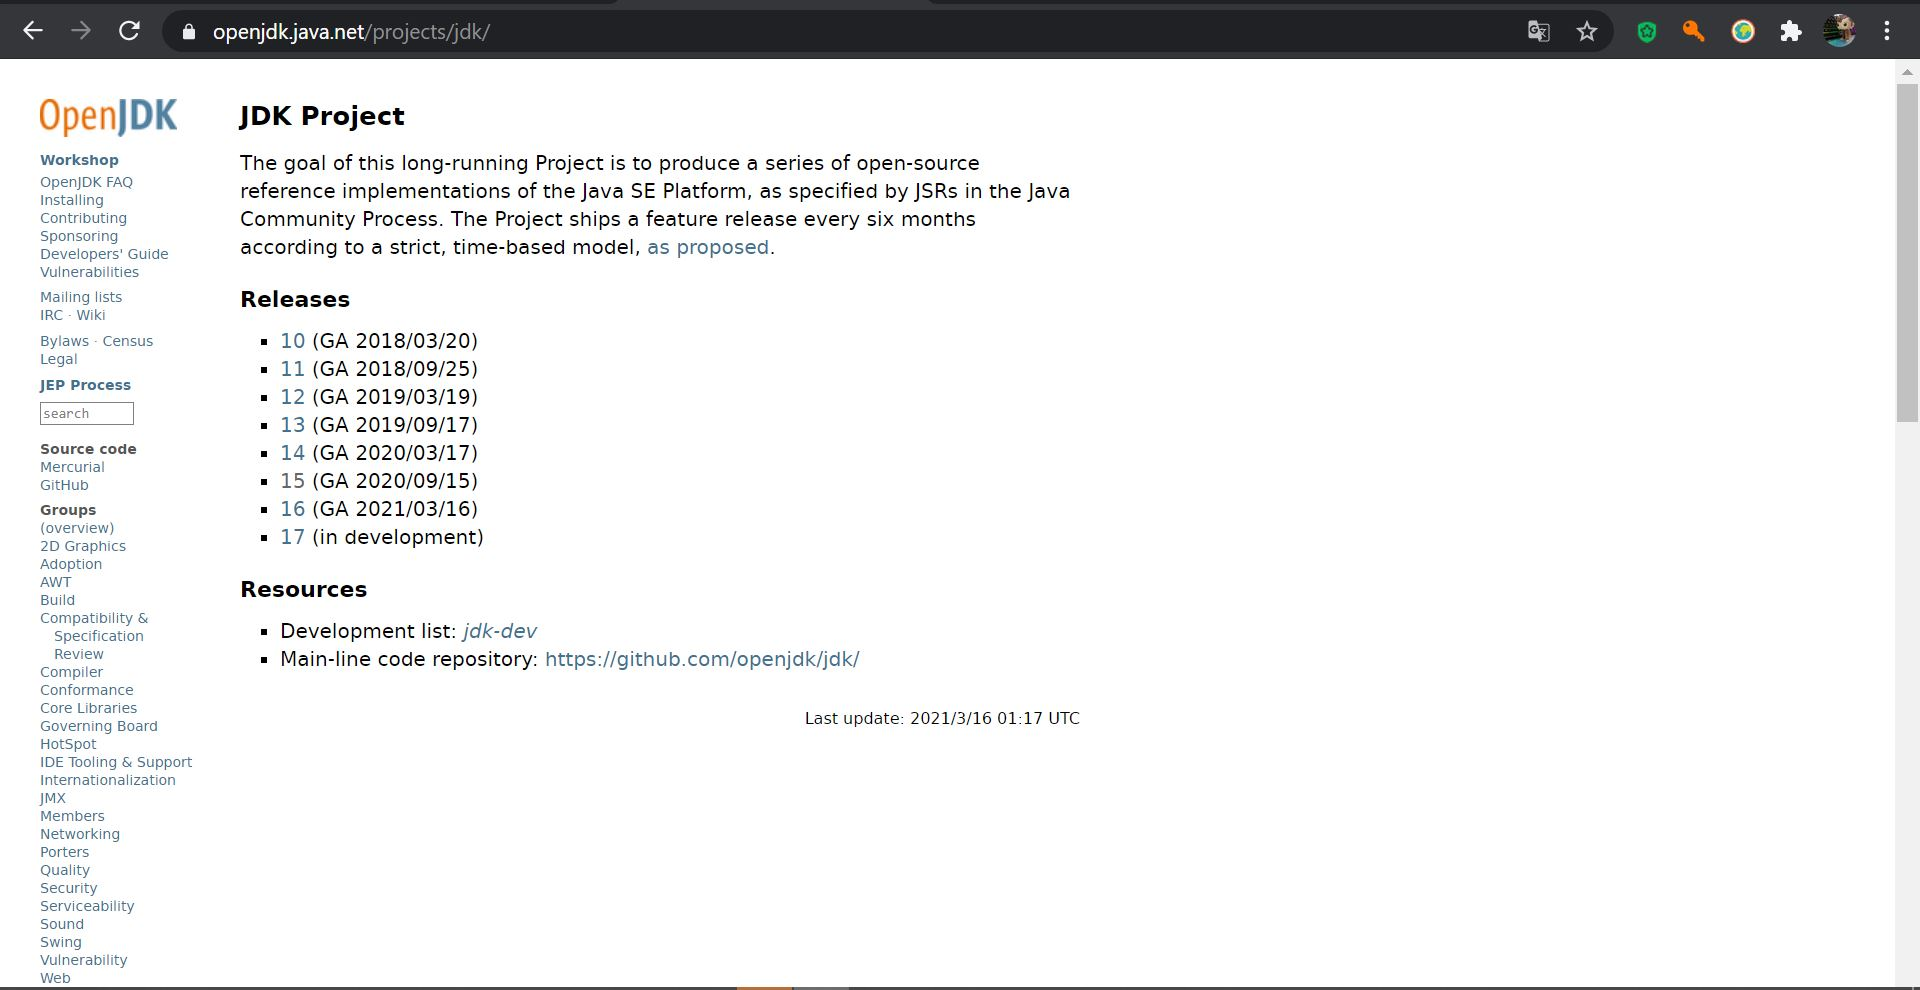
\includegraphics[width=\linewidth]{./img/installation-jdk.JPG}
    \end{center}

    \subsection{Configurer son environnement}
    \begin{enumerate}
        \item Ouvrir le Panneau de configuration Windows
        \item Accéder à la rubrique "Système et sécurité" puis "Système"
        \item Ouvrir la fenêtre "Paramètres système avancés"
        \item Ouvrir la fenêtre "Variable d'environnement"
        \item Sous la rubrique "Variables système", modifier la variable
              \verb|Path| en ajoutant ou modifiant le chemin d'accès au
              jdk-15 ou d'une version ultérieure.
    \end{enumerate}

    \begin{center}
        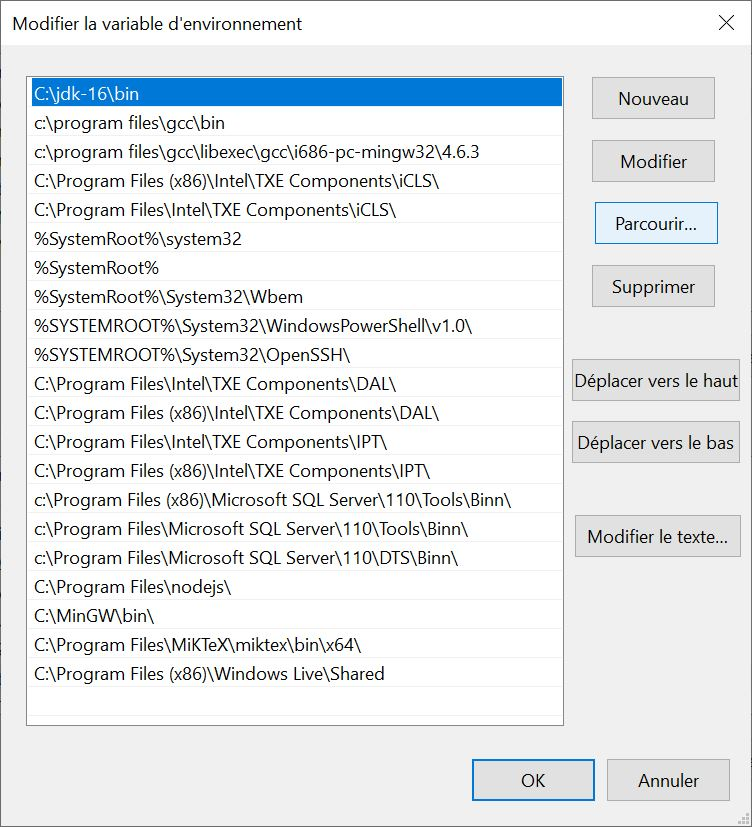
\includegraphics[height=8cm]{./img/installation-variable-environnement.JPG}
    \end{center}

    Pour vérifier de la prise en compte de la variable :
    \begin{enumerate}
        \item Ouvrir un invite de commande
        \item Entrer la commande \verb|javac| suivi de l'option \verb|-version|
    \end{enumerate}


    Exemple :
    \\ \verb|C:\user> javac -version|
    \\ \verb|javac version 15|

\section{Installation de l'Interpréteur LIR}
    Pour installer l'interpréteur LIR, suivre la démarche suivante :
    \begin{enumerate}
        \item Télécharger et ranger le fichier \verb|interpreteurLIR.zip |
              dans son arborescence
        \item Extraire le répertoire \verb|interpreteurLIR| du fichier .ZIP
    \end{enumerate}

    Pour lancer l'interpréteur LIR, il y a plusieurs possibilités :
    \begin{enumerate}
        \item Lancement à partir de l'explorateur de fichiers
        \item Lancement à partir d'un invite de commande
    \end{enumerate}

    \subsection{Lancement à partir de l'explorateur de fichiers}
    Possible si le chemin d'accès (path) au jdk-15 ou une version
    ultérieure est une variable système (cf. Configurer son environnement).
    Dans le répertoire \verb|interpreteurLIR|, sélectionner et ouvrir le fichier
    \verb|lanceInterpreteurLIR.bat|.

    \subsection{Lancement à partir d'un invite de commande}

    Si le chemin d'accès (path) au jdk-15 ou une version ultérieure est
    une variable système n'est pas une variable système, suivre l'étape 2.
    après l'ouverture de l'invite de commande.

    \begin{enumerate}
        \item Ouvrir un invite de commande
        \item \textit{optionnel } Définir une variable d'environnement à l'aide
              de la commande \verb|set path=| suivi du chemin d'accès au répertoire
              \verb|bin| de votre version du jdk.
              \\ Exemple : \verb|C:\user> set path=C:\jdk-15\bin|
        \item À l'aide de la commande \verb|cd| se placer dans le répertoire
              \verb|interpreteurLIR|
        \item Écrire \verb|lanceInterpreteurLIR.bat| ou alors
              \verb|java -jar interpreteurLIR.jar| pour lancer l'interpréteur
    \end{enumerate}

    Exemples 1 de lancement :
    \\ \verb|C:\user> javac -version|
    \\ \verb|javac version 8|
    \\ \verb|C:\user> set path=C:\jdk-15\bin|
    \\ \verb|C:\user>cd C:\user\Documents\chemin_d_acces\interpreteurLIR|
    \\ \verb|C:\user\Documents\chemin_d_acces\interpreteurLIR> lanceInterpreteurLIR.bat| \\
    \\ Exemple 2 de lancement :
    \\ \verb|C:\user> javac -version|
    \\ \verb|javac version 15|
    \\ \verb|C:\user>cd C:\user\Documents\chemin_d_acces\interpreteurLIR|
    \\ \verb|C:\user\Documents\chemin_d_acces\interpreteurLIR> java -jar interpreteurLIR.jar|








    \chapter{Éléments de langage}
        \input{fichiers/elementDeLangage/chapElementsDeLangage.tex}

        \section{Mots-clés}
            % nom du chapitre ici en commentaire
% nom de la section ici en commentaire

\subsection{...} % nom de section
\subsubsection{...}
    \paragraph{...}
    \subparagraph{...}

            \subsection{Commandes générales}
                \begin{description}
	\item[\textbf{Debut :}] Vide l'intégralité du contexte d'exécution.
	
	\item[\textbf{Fin :}] Quitte l'interpréteur.
	
	\item[\textbf{Defs :}] Sert a voir toutes les variables définies dans la session courante\\ (les identificateurs et les valeurs).
	
	\item[\textbf{Lance :}] Exécute le programme chargé en mémoire avec ou sans étiquette.
	
	\item[\textbf{Efface :}] Supprime une ou plusieurs lignes de code suivant les étiquettes \\ début et fin mises en argument.
	
	\item[\textbf{Liste :}] Affiche toutes les lignes de programme mémorisées dans l'ordre\\ croissant entre les numéros de ligne de l'intervalle étiquette début et fin donné en argument. Sans argument Affiche toutes les lignes de \\programme dans l'ordre croissant des numéros de ligne.
	
	\item[\textbf{Sauve :}] Sauvegarde un programme LIR dans un fichier.
	
	\item[\textbf{Charge :}] Charge un programme LIR préalablement enregistré \\ dans un fichier.

\end{description} 

            \subsection{Instructions de programmation}
                \begin{description}
	\item [\textbf{Var :}] Initialise une expression (chaine de caractère ou entier) dans variable définie par son identificateur, aussi utilisé pour changer sa valeur.

	\item [\textbf{Entre :}] Invite l'utilisateur a saisir une expression dans l'entrée standard. Celle-ci sera affectée dans la variable passée en argument.

	\item [\textbf{Affiche :}] Affiche le contenu de l'expression passé en argument sur la console de l'interpreteur. Si il n'y a pas d'argument cela provoque un saut de ligne.

	\item [\textbf{Vaen :}] Effectue un saut dans le programme vers l'étiquette passée en argument.

	\item [\textbf{Si ... vaen :}] Effectue un saut conditionnel, si l'expression booléenne passée en premier argument (entre si et vaen) est vrai, un saut s'effectue à l'étiquette passée en second argument (après vaen). 

	\item [\textbf{Procedure :}] Appel d'une fonction située à l'étiquette spécifiée. Puis reprend l'execution à la suite de cette action.

	\item [\textbf{Retour :}] Défini la fin d'une fonction, ordonne à l'interpreteur de retourner à la suite de l'instruction qui suit son appel.

	\item [\textbf{Stop :}] Arrête le programme.

\end{description}

        \section{Étiquettes}
            % nom du chapitre ici en commentaire
% nom de la section ici en commentaire

\subsection{...} % nom de section
\subsubsection{...}
    \paragraph{...}
    \subparagraph{...}

        \section{Constantes littérales}
             % nom du chapitre ici en commentaire
% nom de la section ici en commentaire

\subsection{...} % nom de section
\subsubsection{...}
    \paragraph{...}
    \subparagraph{...}

             \subsection{Entiers}
                Les valeurs entières sont exprimées en base 10 et donc formées des caractères +, -, 0, 1, 2, 3, 4, 5, 6, 7, 8, 9.\\
Leur valeur est comprise dans l'intervalle [-2\up{31}=-2147483648\verb|,| 2\up{31}=2147483648].


             \subsection{Chaînes de caractères}
                Les chaînes seront entourées de guillemets et limitées à 70 caractères.

        \section{Identificateurs}
             % nom du chapitre ici en commentaire
% nom de la section ici en commentaire

\subsection{...} % nom de section
\subsubsection{...}
    \paragraph{...}
    \subparagraph{...}

             \subsection{Identificateurs d'entiers}
                Les nom identifiants des entiers commenceront obligatoirement par une lettre qui sera suivie d'au plus 24 lettres ou chiffres.

             \subsection{Identificateurs de Chaînes}
                Les noms identifiant des chaînes de caractères commenceront par le symbole \$, suivi d'une lettre, qui sera suivie d'au plus 24 lettres ou chiffres.

        \section{Expressions}
            % nom du chapitre ici en commentaire
% nom de la section ici en commentaire

\subsection{...} % nom de section
\subsubsection{...}
    \paragraph{...}
    \subparagraph{...}

            \subsection{Expression entière}
                Les expressions concernent toujours deux opérandes séparés par un opérateur (notation infixe).
La présence d’espace (séparateur neutre) n’est pas obligatoire (mais conseillée).
Un opérande est soit une constante littérale, soit un identificateur.
L’opérateur est un caractère symbolisant les opérations arithmétiques courantes : +, -, *, /, \% \\

\begin{description}
	\item \verb|+|: addition entière
	\item \verb|-|: soustraction entière
	\item \verb|*|: multiplication entière
	\item \verb|/|: quotient de la division entière
	\item \verb|%|: reste de la division entière 
\end{description}

            \subsection{Expression sur chaînes}
                La seule opération utilisée sur les chaînes est la concaténation.
Composée de 2 opérandes chaînes, c’est-à-dire des constantes chaînes ou identificateurs commençant par \$.

            \subsection{Conditions}
                Les expressions logiques ne sont utilisées qu'avec l'instruction si.
Les expressions logiques concernent donc toujours deux opérandes séparés par un opérateur relationnel (notation infixe).
Un opérande est soit une constante, soit un identificateur.
L’opérateur relationnel oprel est un symbole parmi : =, <>, <, <=, >, >= \\

\begin{description}
	\item \verb |=| : représente le test d’égalité
	\item \verb |<>| : représente l’inégalité
	\item \verb |<| : infériorité stricte
	\item \verb |>| : supériorité stricte
	\item \verb |<=| : inférieur ou égal
	\item \verb |=>| : supérieur ou égal
\end{description}

Ces opérateurs ont le sens habituel pour les entiers.
Pour les chaînes, c'est l'ordre lexicographique habituel qui sera utilisé. \\

    \chapter{Utilisation}
        \input{fichiers/utilisation/chapUtilisation.tex}

        \section{Utilisation des commandes et instructions}
            % nom du chapitre ici en commentaire
% nom de la section ici en commentaire

\subsection{...} % nom de section
\subsubsection{...}
    \paragraph{...}
    \subparagraph{...}

            \subsection{Commandes}
                \begin{description}
	\item[\textbf{Debut :}] Sur un programme chargé en mémoire centrale j'efface toutes les lignes de code et variables déclarées avec la commande \verb|debut|.
	
	\item[\textbf{Fin :}] Je suis en train d'utiliser l'interpréteur, je quitte l'interpréteur pour la session courante en exécutant la commande \verb|fin|.
	
	\item[\textbf{Defs :}] Les variables sont définies dans la session courante de l'interpréteur j'affiche le contexte actuel en exécutant la commande \verb|defs|.
	
	\item[\textbf{Lance :}] A partir de lignes d'instructions chargées dans la session courante de l'interpréteur LIR lorsque j'entre la commande \verb|lance| sans arguments et la valide, le programme s'exécute à partir de l'étiquette la plus petite.\\
	 Et avec argument les lignes d'instructions chargées dans la session courante de l'interpréteur LIR et lorsque j'entre la commande \verb|lance| sans arguments et la valide le programme s'exécute à partir de l'étiquette passé en argument.\\
	
	Exemple : \verb|lance| <étiquette début> : <étiquette fin>
	
	\item[\textbf{Efface :}] A partir d'une ou plusieurs lignes de programme mémorisées et leur étiquettes\\ on tape la commande: \verb|efface| <étiquette début> : <étiquette fin>.\\
	L'interpréteur effacera alors les lignes de programme dont le numéro d'étiquette est compris dans la plage.
	
	\item[\textbf{Liste :}]  J'entre la commande \verb| liste <etiquette_debut>:<etiquette_fin> | l'interpréteur va afficher toutes les lignes de programme mémorisées, dans l'ordre croissant de leur étiquette et dont les étiquettes sont situées dans cet intervalle donné. Et sans argument la commande \verb| liste | affiche toutes les lignes de programme mémorisées, dans l'ordre croissant de leur étiquette.
	
	\item[\textbf{Sauve :}] Quand programme (avec des étiquettes) ai été saisi, lorsque on entre la commande \verb|sauve| avec en argument le chemin du fichier (dans lequel on souhaite sauvegarder le travail),
	\verb|sauve <cheminFichier>| les lignes de codes tapées dans l'interpréteur s'enregistres dans le fichier passé en argument de la commande
	pour pouvoir être rechargées plus tard par l'interpréteur LIR avec la commande \verb|charge <cheminFichier>|.
	
	
	
	\item[\textbf{Charge :}] On a un fichier contenant un programme LIR dans notre ordinateur lorsque j'entre la commande \verb|charge| avec en argument le chemin de ce fichier les lignes de codes enregistrées dans le fichier sont chargée dans le
	programme pour pouvoir être exécutées et/ou modifiées par l'interpréteur LIR.
	
	Exemple : \verb|sauve <D:\leCheminDuFichier\leFichier.LextensionDuFichier>| OU \verb|sauve <leFichier.LextensionDuFichier>|
	
\end{description} 

            \subsection{Instructions}
            \begin{description}
	\item [\textbf{Var :}] L'interpréteur enregistre dans la variable spécifiée l'expression.\\
	Syntaxe :
	\verb|<etiquette> var <identificateur> = <expression>|\\

	Exemple: \\
	Pour une variable de chaine de caractère :
	\verb|5 var $varChaine = "chaine"| \\
	Pour une variable d'entier :
	\verb|5 var varEntier = 42| 

	\item [\textbf{Entre :}] Lorsque la valeur est saisie, elle est stockée dans la variable déterminée dans dans le contexte, sous réserve que les types concordes.\\
	Syntaxe :
	\verb|<etiquette> entre <identificateur>|\\

	Exemple: \\
	Pour une variable de chaine de caractère :
	\verb|10 entre $varChaine| \\
	Pour une variable d'entier :
	\verb|10 entre varEntier|

	\item [\textbf{Affiche :}] L'interpréteur évalue dans l'expression spécifiée la valeur de celle-ci et renvoie cette valeur sur la console. Si cette commande n'as pas d'argument elle effectue un saut de ligne.\\
	Syntaxe :
	\verb|<etiquette> affiche [identificateur]|\\

	Exemple: \\
	Sans argument:
	\verb|15 affiche|\\
	Pour une variable de chaine de caractère (\$varChaine = une):
	\verb|15 affiche $varChaine| \\
	Pour une variable d'entier (varEntier = 12):
	\verb|15 affiche varEntier + 5|

	\item [\textbf{Vaen :}] Lors de l'exécution de l'instruction, le programme ignorera les lignes suivantes et sautera directement à la ligne indiquée.\\
	Syntaxe :
	\verb|<etiquette> vaen <etiquette>|\\

	Exemple: \verb|20 vaen 30|

	\item [\textbf{Si ... vaen :}] Lors de l'execution de l'instruction, le programme igorera les lignes suivantes et sautera directement à la ligne indiquée si et seulement si la condition (booléenne) imposée est valide.\\
	Syntaxe :
	\verb|<etiquette> si <condition> vaen <etiquette>|\\

	Exemple: \verb|25 si varEntier <> 8 vaen 35|

	\item [\textbf{Procedure :}] L'interpréteur vas chercher la ligne qui a pour identificateur celui référencé en étiquette et vas l'exéctuer jusqu'à la fin de la séquence.\\
	Syntaxe :
	\verb|<etiquette> procedure <etiquette>|\\

	Exemple: \verb|30 procedure 60|

	\item [\textbf{Retour :}] L'interpréteur vas chercher la ligne qui suivait l'instruction "procedure" et va l'exécuter jusqu'à la fin de la séquence.\\
	Syntaxe :
	\verb|<etiquette> retour|\\

	Exemple: \verb|70 retour|

	\item [\textbf{Stop :}] A son exécution, le programme s'arrête lorsqu'il a atteint l'étiquette spécifiée.\\
	Syntaxe :
	\verb|<etiquette> stop|\\

	Exemple: \verb|40 stop|
\end{description}

        \section{Programmation en LIR}
            La programmation en LIR peut s'effectuer de deux manières :
\begin{enumerate}
	\item \textbf{Programmation directement dans l'interpréteur.} Celle-ci s'effectue en ajoutant une étiquette, donnant l'ordre d'exécution, avant l'instruction saisie. Les lignes de code peuvent être ajoutés dans le désordre dans le programme chargé. Le remplacement d'une instruction à une certaine étiquette se fait par la saisie d'une ligne de code ayant la même étiquette. Les commandes liste et efface permettent l'édition du programme.
	\item \textbf{Programmation dans un fichier d'extension .lir} qui sera chargé à posteriori dans l'interpréteur avec la commande charge. Une ligne saisie dans le fichier correspond à une saisie dans l'interpréteur ainsi les mêmes spécificité s'appliquent. Une ligne invalide empêche le chargement de l'entièreté du fichier. Les lignes blanches sont ignorées par l'interpréteur.
\end{enumerate}
Ces deux méthodes se complètent grâce aux commandes sauve et charge permettant de passer d'une méthode à l'autre.

    \chapter{Exemples d'utilisation}
        Exemples d'utilisation de l'interpréteur LIR :
\begin{verbatim}
Interpréteur Langage IUT de Rodez, bienvenue !
Entrez vos commandes et instructions après l’invite ? 

? defs
aucune variable n'est définie
? liste
aucune ligne à afficher
? 10 var $message = "Hello World !"
ok
? 20 afficher $message
nok : mot clé inconnu
? 20 affiche message
ok
? 20 affiche $message
ok
? liste
10 var $message = "Hello World !"
20 affiche $message
? liste 20:20
20 affiche $message
? 15 stop
ok
? liste
10 var $message = "Hello World !"
15 stop
20 affiche $message
? efface 11:19
ok
? liste
10 var $message = "Hello World !"
20 affiche $message
? 30 stop
ok
? lance
Hello World !
? sauve helloWorld.lir
ok
? defs
$message = "Hello World !"
? liste
10 var $message = "Hello World !"
20 affiche $message
30 stop
? debut
ok
? defs
aucune variable n'est définie
? liste
aucune ligne à afficher
? charge helloWorld.lir
ok
? liste
10 var $message = "Hello World !"
20 affiche $message
30 stop
? var $message = "Aurevoir !"
ok
? lance 20
Aurevoir !
? fin
Au revoir, à bientôt !
\end{verbatim}

Exemples de programmes en LIR :
\begin{enumerate}
	\item \textbf{Exemple d'un programme demandant un état civil simple : }
\begin{verbatim}
10 affiche "Entre ton nom : " 
20 entre $nom 
30 affiche "Bienvenue "+$nom 
35 affiche 
40 var an=2021 
50 affiche "Quelle est ton année de naissance ? " 
60 entre naissance 
65 si naissance > an vaen 50 
70 affiche "Tu as autour de " 
80 affiche an-naissance 
90 affiche "ans " 
100 affiche 
200 stop
\end{verbatim}
    \underline{Exemple d'exécution :}
\begin{verbatim}
? charge etatCivilSimple.lir
ok
? lance
Entre ton nom : Emmanuel MACRON
Bienvenue Emmanuel MACRON
Quelle est ton année de naissance ? 1977
Tu as autour de 44ans 
\end{verbatim}
    \item \textbf{Exemple d'un programme calculant la factorielle à partir d'un entier saisi par l'utilisateur :}
\begin{verbatim}
10 affiche "Bienvenue dans le programme factorielle.lir !"
20 affiche
30 affiche "Entrez un entier : "
40 entre entier
45 procedure 500
50 procedure 1000
60 affiche entier
70 affiche "! = "
80 affiche factorielle
90 affiche
200 stop
    		
500 si entier >= 0 vaen 600
510 affiche "n! est définie sur l'ensemble des entiers naturels"
520 stop
600 retour 

1000 var factorielle = 1
1010 var entierCourant = 2
1011 var ancienFactorielle = factorielle
1012 var test = factorielle
1015 si entierCourant > entier vaen 1100
1016 si ancienFactorielle <> test vaen 1060
1017 var ancienFactorielle = factorielle
1020 var factorielle = factorielle * entierCourant
1025 var test = factorielle / entierCourant
1030 var entierCourant = entierCourant + 1
1040 vaen 1015
1050 vaen 1100
1060 affiche "dépassement de la capacité des entiers pour "
1070 affiche entier
1080 affiche "!"
1090 affiche
1095 stop
1100 retour
\end{verbatim}
    \underline{Exemple d'exécution :}
\begin{verbatim}
? charge factorielle.lir
ok
? lance
Bienvenue dans le programme factorielle.lir !
Entrez un entier : 10
10! = 3628800
\end{verbatim}
    \item \textbf{Exemple d'un programme déterminant l'entier médian de 3 entiers saisis :}
\begin{verbatim}
10 affiche "Bienvenue dans le programme Median3Entiers.lir"
20 affiche
30 affiche "Entrez le premier entier : "
40 entre premier
50 affiche "Entrez le deuxième entier : "
60 entre deuxieme
70 affiche "Entrez le troisième entier : "
80 entre troisieme
90 procedure 1000
100 affiche "Median( "
110 affiche premier
120 affiche ", "
130 affiche deuxieme
140 affiche ", "
150 affiche troisieme
160 affiche ") = "
170 affiche median
180 affiche
250 stop
        
1000 si premier <= deuxieme vaen 1100
1010 si deuxieme <= troisieme vaen 1200
1020 vaen 1520
        
1100 si deuxieme <= troisieme vaen 1520
1110 si premier <= troisieme vaen 1540
1120 vaen 1500
        
1200 si premier <= troisieme vaen 1500
1220 vaen 1540

1500 var median = premier
1510 vaen 1550
1520 var median = deuxieme
1530 vaen 1550
1540 var median = troisieme
1550 retour
\end{verbatim}
    \underline{Exemple d'exécution :}
\begin{verbatim}
? charge Median3Entiers.lir
ok
? lance
Bienvenue dans le programme Median3Entiers.lir
Entrez le premier entier : 55
Entrez le deuxième entier : 27
Entrez le troisième entier : 96
Median( 55, 27, 96) = 55
\end{verbatim}
\end{enumerate}



\end{document}